\documentclass[12pt,a4paper,twoside]{book}
\usepackage{graphicx}
\usepackage{setspace}	%double spacing for text, single for captions, footnotes, etc.
%\usepackage{hypernat} 	%substitut de cite que permet fer hyperlinks
\usepackage{natbib}		% substituye a 'hypernat' que funciona en Windows.
\usepackage[spanish]{babel}
\usepackage[utf8]{inputenc}
\usepackage{color}
\usepackage{hhline} 		% extended styles for tables
\usepackage{multirow}
\usepackage{subfigure}
\usepackage{acronym}
\usepackage{hyperref}
\usepackage{amsmath,amsmath,amssymb} 
\usepackage{fancyhdr}
\usepackage{epsfig, amsmath}
\usepackage{algorithm}
\usepackage{algorithmic}
\usepackage{epigraph}
\usepackage{titlesec}


% general settings
\hypersetup{
	linktocpage=true,
	colorlinks=true,
	linkcolor=blue,
	citecolor=blue,
}
\definecolor{Hgray}{gray}{0.6}

\newenvironment{definition}[1][Definition]{\begin{trivlist}
\item[\hskip \labelsep {\bfseries #1}]}{\end{trivlist}}

\setlength{\topmargin}{0cm}
\setlength{\textheight}{23cm}
\setlength{\textwidth}{17cm}
\setlength{\oddsidemargin}{0cm}
\setlength{\evensidemargin}{0cm}
\setlength{\headheight}{1cm}
\setlength{\parskip}{0.5cm}

% indica que las 'sub-sub-sections' sean numeradas y aparezcan en el indice
\setcounter{secnumdepth}{3}
\setcounter{tocdepth}{2}

% settings for code
\renewcommand{\algorithmicrequire}{\textbf{Entrada: }}
\renewcommand{\algorithmicensure}{\textbf{Salida: }}
%\newcommand{\sectionbreak}{\clearpage}

%%%%%%%%%%%%
% DOCUMENT %
%%%%%%%%%%%%
\begin{document}

% portada
\newpage
\thispagestyle{empty}

\baselineskip 2em

%\vspace*{1cm}

\centerline{
\includegraphics[width=0.6\textwidth]{images/UOC-logo}}
\begin{center}
\textsc{Universitat Oberta de Catalunya (UOC) \\
 Máster Universitario en Ciencia de Datos (\textit{Data Science})\\}

%\centerline {\pic{UOC}{4cm}}

\vspace*{1.5cm}

\textsc{\Large TRABAJO FINAL DE MÁSTER}

\vspace*{0.5cm}

\textsc{\large Área: Minería de datos y Machine Learning}


%\textbf{\Huge VirtualTechLab Model: }

\vspace*{2.0cm}

\textbf{\Large Detección de anomalías en entorno del Internet de las cosas}


\vspace{2.5cm}
\baselineskip 1em

\baselineskip 2em
-----------------------------------------------------------------------------\\
Autor:      Gonzalo Pedro Mellizo-Soto Díaz\\
Tutor:      Carlos Hernández Gañán \\
Profesor:   Jordi Casas Roma \\
-----------------------------------------------------------------------------\\
\vspace*{1.5cm}
Madrid, \today

\end{center}

\newpage
\pagestyle{empty}
\hfill

\newpage
% abstract
\pagenumbering{roman} 
\setcounter{page}{1} 
\pagestyle{plain}

%%%%%%%%%%%%%%%%
%%% CREDITOS %%%
%%%%%%%%%%%%%%%%
\chapter*{Copyright}

\vspace{1cm}

\begin{figure}[ht]
    \centering
	
\includegraphics[scale=1]{images/license.png}
\end{figure}

Esta obra está sujeta a una licencia de Reconocimiento -  NoComercial - SinObraDerivada

\href{https://creativecommons.org/licenses/by-nc-nd/3.0/es/}{3.0 España de CreativeCommons}.

%%%%%%%%%%%%%
%%% FICHA %%%
%%%%%%%%%%%%%
\chapter*{FICHA DEL TRABAJO FINAL}

\begin{table}[ht]
	\centering{}
	\renewcommand{\arraystretch}{2}
	\begin{tabular}{r | l}
		\hline
		Título del trabajo: & Detección de anomalías en el entorno del Internet de las cosas\\
		\hline
        Nombre del autor: & Gonzalo Pedro Mellizo-Soto Díaz\\
		\hline
        Nombre del colaborador/a docente: & Carlos Hernández Gañán\\
		\hline
        Nombre del PRA: & Jordi Casas Roma\\
		\hline
        Fecha de entrega (mm/aaaa): & 06/2019\\
		\hline
        Titulación o programa: & Máster Universitario en Ciencia de Datos\\
		\hline
        Área del Trabajo Final: & Minería de datos y Machine Learning \\
		\hline
        Idioma del trabajo: & Español\\
		\hline
        Palabras clave & Machine Learning, IOT, Anomaly Detection\\
		\hline
	\end{tabular}
\end{table}

%%%%%%%%%%%%%%%%%%%
%%% DEDICATORIA %%%
%%%%%%%%%%%%%%%%%%%
\chapter*{Cita}

\setlength\epigraphwidth{.8\textwidth}
\setlength\epigraphrule{0pt}

\epigraph{\itshape``Nuestro lema es: más humanos que los humanos"}{Eldon Tyrell, \textit{Blade Runner}}

%%%%%%%%%%%%%%%%%%%
%%% Agradecimientos %%%
%%%%%%%%%%%%%%%%%%%
\chapter*{Agradecimientos}

TO BE DEFINED

Si se considera oportuno, mencionar a las personas, empresas o instituciones que hayan contribuido en la realización de este proyecto.

%%%%%%%%%%%%%%%%
%%% RESUMEN  %%%
%%%%%%%%%%%%%%%%
\chapter*{Abstract}
\addcontentsline{toc}{chapter}{Abstract}

\onehalfspacing

In recent years the amount of connected devices has greatly increased, with an increasing number of applications in the industry each day. This devices can be subject of attacks causing instability or data leaks that can be dangerous both for the users and the enterprises, in order to avoid or confront them, security and early detection are becoming a must in a connected world. The focus is the monitoring and detection of the attacks in Internet of Things devices using state of the art Machine Learning techniques. Models such as SVM, DBScan or Isolation Forests have been used and assembled in order to identify with a better accuracy when an attack is happening. With this assembly, attack detection has increased up to 15\% comparing to traditional methods and individual model usages and times have been considerably reduced. An active use of Machine Learning models has shown a great improvement at anomaly detection by securing the devices and decreasing the reaction times when facing attacks.

\vspace{0.5cm}

Durante los últimos años se encuentra una creciente cantidad de dispositivos conectados entre sí, cada vez con más aplicaciones en la industria. Estos dispositivos pueden ser atacados y provocar inestabilidad o una fuga de datos, por lo tanto la protección y la pronta detección de ataques y/o anomalías es vital en un mundo cada vez más conectado. El objetivo es la monitorización y detección de estos ataques en dispositivos del \textit{Internet of Things} utilizando técnicas del estado del arte de Machine Learning para su detección y poder así responder con una mayor rapidez a los ataques. Para la detección se han utilizado modelos estadísticos, como SVM, DBScan o Isolation Forests, que en su conjunto permitan identificar con mayor precisión cuando se está produciendo un ataque. El conjunto de la clusterización con la clasificación de puntos anómalos muestra una mayor robustez, frente al uso individual de cada uno de los modelos aumentando la detección en hasta un 15\%. Se demuestra cómo el uso de los modelos permite proteger los dispositivos y mejorar la seguridad al disminuir los tiempos de reacción frente a los ataques.

\vspace{0.5cm}
\textbf{Palabras clave}: Machine Learning, IOT, Anomaly Detection
\newpage

\pagestyle{fancy}
\renewcommand{\chaptermark}[1]{ \markboth{#1}{}}
\renewcommand{\sectionmark}[1]{\markright{ \thesection.\ #1}}
\lhead[\fancyplain{}{\bfseries\thepage}]{\fancyplain{}{\bfseries\rightmark}}
\rhead[\fancyplain{}{\bfseries\leftmark}]{\fancyplain{}{\bfseries\thepage}}
\cfoot{}

% indice
\cleardoublepage
\phantomsection
\addcontentsline{toc}{chapter}{Índice}
\tableofcontents
% listado de figuras
\cleardoublepage
\phantomsection
\addcontentsline{toc}{chapter}{Listado de Figuras}
\listoffigures
% listado de tablas
\cleardoublepage
\phantomsection
\addcontentsline{toc}{chapter}{Listado de Tablas}
\listoftables

\thispagestyle{empty}

\pagenumbering{arabic}

\pagestyle{fancy}
\renewcommand{\chaptermark}[1]{ \markboth{#1}{}}
\renewcommand{\sectionmark}[1]{\markright{ \thesection.\ #1}}
\lhead[\fancyplain{}{\bfseries\thepage}]{\fancyplain{}{\bfseries\rightmark}}
\rhead[\fancyplain{}{\bfseries\leftmark}]{\fancyplain{}{\bfseries\thepage}}
\cfoot{}

\onehalfspacing

% capitulos del documento
\chapter{Introducción}
\label{chapter:introduccion}


%%% SECTION
\section{Contexto y justificación del Trabajo}
Cada vez se encuentran más dispositivos conectados entre sí no solo en la industria, si no también en los hogares, esta conexión entre dispositivos los hace vulnerables a ataques informáticos que pueden afectar en gran medida a los usuarios, no solo pueden provocar un mal funcionamiento de los mismos, si no que también puede provocar la fuga de datos de distinta sensibilidad. La previsión en los futuros años es de cada vez estar más conectados y una pronta detección de los ataques puedo ayudar a evitar los problemas derivados de los mismos, mediante una pronta reacción o frente a la previsión de un ataque.

\vspace{0.5cm}

Actualmente se utilizan distintas medidas de seguridad como control de acceso físico al dispositivo, encriptación de datos, firewalls, securización de red, etc... Sin embargo, en muchos casos la detección de anomalías aplican un umbral estacionario, provocando que en el caso de un ataque ya sea demasiado tarde para reaccionar o no sean capaz de identificar patrones extraños previos al ataque. Con la aplicación de nuevas técnicas se pretende mejorar los tiempos de reacción e incluso predecir cuándo puede suceder un ataque.

\section{Explicación de la motivación personal}
La razón principal de la selección del proyecto es la posibilidad de aprender y utilizar técnicas de Machine Learning en un sector desconocido que permita diversificar conocimientos. Cada vez más todo se encuentra conectado e investigar cómo clasificar cuando se está produciendo un ataque permite profundizar en conocimientos de seguridad y aplicarlos en un problema real.

\vspace{0.5cm}

La aplicación de técnicas en un problema real ayuda a comprender mejor el uso de las herramientas y el por qué y cuándo se deben de utilizar. De este modo, se añade un nuevo conocimiento que puede aportar en el ámbito profesional y puede utilizarse también en un entorno privado.


\section{Objetivos del Trabajo}
Los objetivos del trabajo son los siguientes:

\begin{itemize}
  \item Adquisición de conocimiento del sector y de los dispositivos IOT
  \item Lectura y comprensión de las técnicas del estado del arte en detección de anomalías en dispositivos conectados.
  \item Obtención de datos reales de conexiones a dispositivos IOT, en caso de no ser posible, generación de datos sintéticos.
  \item Prueba de las técnicas encontradas y evaluación en el problema actual.
  \item Investigación de algoritmos tradicionales de Machine Learning y su utilidad en el problema actual.
  \item Desarrollo de la solución utilizando los algoritmos más aptos.
  \item Evaluación de la detección de patrones y ataques de las técnicas utilizadas.
  \item Comparar los resultados obtenidos con el estado del arte y probar si existen mejoras frente a los métodos actuales.
\end{itemize}

\section{Descripción general del problema}

En la actualidad, la cantidad de dispositivos informáticos existentes que pueden ser víctimas de un ataques es masiva, por lo que securizar bien los dispositivos es fundamental. A pesar de el uso de distintos protocolos de seguridad, se generan nuevos tipos de ataque todos los días, por lo tanto la detección es una necesidad para evitar los problemas derivados.

\vspace{0.5cm}

La pérdida de control de los dispositivos o la fuga de información de los mismos puede provocar pérdidas millonarias a las empresas o provocar una gran inseguridad a los usuarios de productos IOT, así como provocar posibles daño a infraestructuras o personas. Por otro lado, muchos de los dispositivos pueden no tener la capacidad de computación necesaria para incluir una capa de seguridad robusta, que puede compensarse con una detección temprana. 


\section{Enfoque y método seguido}
El enfoque es aplicado al conocer el problema y se intenta dar respuesta a preguntas específicas, mediante la aplicación de los conocimientos obtenidos y la evaluación de la propia aplicación de los mismos.  \par

\vspace{0.5cm}

El método seguido del desarrollo se va a implementar dentro del marco de trabajo \textit{Agile} pensando el desarrollo de la solución como un producto, de este modo se podrá iterar sobre una arquitectura definida y enfocarse en el desarrollo del producto en su total, frente a un modelo tradicional de cascada donde cada fase de desarrollo recae en una sola parte del total.

\vspace{0.5cm}

El formato de entrega será mediante un \textit{minimum viable product} (MVP) en sprints de dos semanas durante el periodo de desarrollo y evaluación de las necesidades según la evolución del producto.

\section{Planificación del Trabajo}

Para la planificación del trabajo se han subdividido las tareas principales y se han mostrado en el siguiente diagrama de Gantt \ref{fig:gantt}.

\begin{itemize}
    \item Pec01 - Definición
    \item Pec01 - Planificación
    \item Pec02 - Búsqueda de fuentes del estado del arte
    \item Pec02 - Lectura de estado del arte
    \item Pec02 - Justificación de estado del arte
    \item Pec02 - Redacción
    \item Pec02 - Refinamiento de objetivos
    \item Pec03 - Planificación de Sprints
    \item Pec03 - Sprint 1
    \item Pec03 - Sprint 2
    \item Pec03 - Sprint 3
    \item Pec03 - Refinamiento/Redacción
    \item Pec04 - Revisión apartados anteriores
    \item Pec04 - Redacción nuevos apartados
    \item Pec05 - Presentación y defensa
\end{itemize}



\begin{figure}[h]
	\centering
	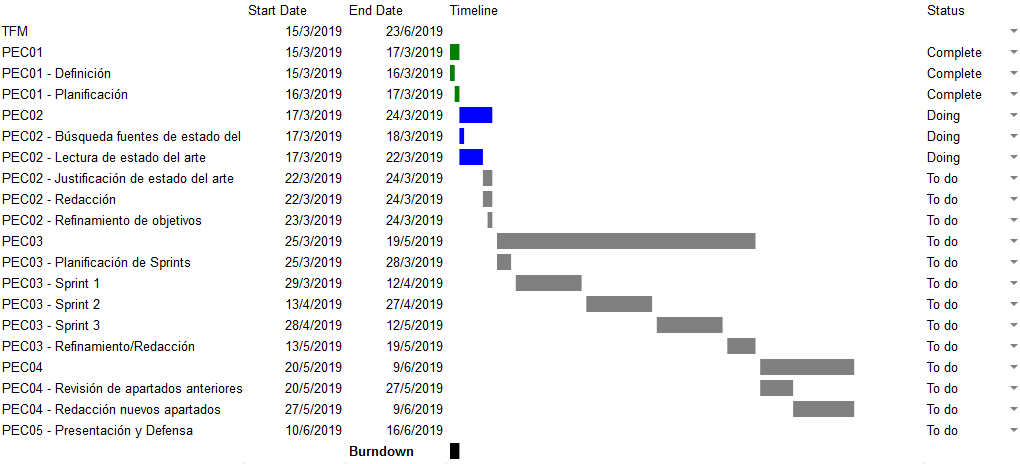
\includegraphics[width=1\textwidth]{figs/gantt_init.PNG}
	\caption{Planificación de tareas}
	\label{fig:gantt}
\end{figure}

\newpage
\chapter{Estado del Arte}
\label{chapter:Estado del Arte}

Una de las aplicaciones más comunes dentro de la detección de anomalías es para la detección de intrusos (\textit{Intrusion Detection}) y la creación de sistemas de detección de intrusos (\textit{Intrusion Detection System, IDS}). Se trata de sistemas cuyo objetivo es la monitorización de los sistemas y redes informáticas, con el fin de alertar en caso de que puedan existir brechas de seguridad\cite{intrusionSystems}. 

Con la ingente cantidad de redes y sistemas que se pueden encontrar a día de hoy es necesario incluir uno de estos sistemas, con el fin de mantener la integridad y disponibilidad de los mismos. Dentro de los IDS, se pueden identificar dos grandes implementaciones de estos sistemas, en los sistemas de detección de intrusos en Host (\textit{Host-Based Intrusion Detection Systems, HIDS}) y los sistemas de detección de intrusos en red (\textit{Network Intrusion Detection Systems, NIDS}).

\begin{itemize}
    \item \textbf{HIDS:} Estos sistemas se caracterizan por implementarse en el Host utilizando información del propio sistema operativo para detectar actos maliciosos \cite{HIDS}. Esta información tiene distintos niveles de información, pero por lo general tienden a ser de bajo nivel sobre operaciones que se pueden estar realizando dentro del sistema. Esta información se consulta dentro de logs, por lo que el análisis de la información es más lento.
   \item \textbf{NIDS:} Para el segundo caso la monitorización se realiza a sistema de red, es decir, de comunicaciones entre distintos nodos y la monitorización de los paquetes que viajan entre ellos \cite{intrusionSystems}. Esta información puede ser consumida en tiempo real, por lo que la reacción ante algún evento es más rápida que en los HIDS que necesitan revisar las acciones.
\end{itemize}

%%% SECTION
\section{Métodos tradicionales de detección de anomalías}
En la sección actual se describen algunos de los métodos tradicionales utilizados en IDS, tanto para HIDS como para NIDS.

\begin{itemize}
    \item Network Security Monitor (NSM):  se trata de uno de los primeros sistemas que permitió auditar el tráfico que circulaba dentro de la red \cite{surveyIDS}. El sistema escucha pasivamente dentro de la red y detecta si existe una conducta sospechosa al desviarse de patrones de conducta. La mayor parte de la monitorización se basa en protocolos estándar como \textit{telnet, ftp, TCP/IP, etc.} por lo que le permitía utilizar una gran cantidad de datos heterogéneos.
    \item State transition analysis (USTAT): el sistema parte de que el host en un momento se encuentra en un estado seguro y que según las acciones que se realizan sobre el mismo el host cambia de estado, hasta que llega a un estado en el que compromete la seguridad \cite{surveyIDS}. Este sistema analiza los estados por los que ha pasado la máquina desde el estado seguro al comprometido. 
    \item GrIDS: se trata de un IDS que utiliza un sistema de construcción de grafos basados en la red, donde cada nodo representa a un host y las aristas las conexiones entre los mismos. La representación gráfica de la actividad de la red permite ayudar al espectador en identificar qué está sucediendo \cite{surveyIDS}.
    \item Haystack: en este caso el IDS se ayuda de métodos estadísticos para la detección de anomalías, definiendo estrategias para usuarios y grupos, además de definir variables del modelo como variables gaussianas independientes \cite{garcia2009anomaly}. Para la detección se incluyen una serie de intervalos en los valores que en el momento que salen del rango normal, se calcula la distribución de probabilidades y si el \textit{score} o puntuación es demasiado grande se genera una alerta.
\end{itemize}

Los métodos/sistemas listados se desarrollaron durante los años noventa, la tecnología ha evolucionado desde entonces y los sistemas se han vuelto más complejos y más propensos a los ciberataques. Por ello, se han desarrollado nuevas técnicas que se apoyan en el uso de técnicas de minería de datos (\textit{Data Mining}) y las técnicas que se describirán a continuación de \textit{Machine Learning}.

\section{Machine Learning y la detección anomalías}

El \textit{Machine Learning} es una rama de la inteligencia artificial cuya premisa es hacer que la máquina aprenda una tarea sin haber sido específicamente programada para ello. El término fue descrito por Arthur L. Samuel en 1959 en un artículo en el que explica estudios de \textit{Machine Learning} aplicado al juego de las damas \cite{samuel2000some}, utilizando en una primera instancia métodos de aprendizajes más generales, como las redes neuronales de las que hablaremos más adelante, y otro métodos que tendrán que ser parametrizados para sus distintos usos.

La inteligencia artificial se puede entender como la inteligencia ejercida por las máquinas, al contrario que la inteligencia natural inherente a los humanos, que son capaces de realizar tareas cognitivas que permiten potenciar la resolución de las mismas e imitar comportamientos como el aprendizaje \cite{russell2016artificial}. Dentro de la inteligencia artificial se pueden encontrar distintas definiciones según si se centran en el razonamiento o en el comportamiento:

\begin{itemize}
    \item Actuar humanamente: este enfoque se basa en que las máquinas actúen como humanos más centrado en la interacción de máquinas con personas, más que en la resolución de problemas. Esta interacción se puede ver reflejada en el test ideado por Alan Turing en 1950, en el que se somete a la máquina "inteligente" a un interrogatorio realizado por un humano, donde éste no sabe que está hablando con una máquina, por lo tanto si es incapaz de detectar que se trata de una máquina esta ha actuado como un humano y puede considerarse inteligente.
    \item Pensar humanamente: esta vertiente se centra en imitar el pensamiento humano, entender cómo funcionan las mentes de los mismos y replicarlo en máquinas. Siguiendo esta corriente, si se consigue imitar el pensamiento humano, una máquina que resuelva el problema utilizará razonamientos humanos, en lugar de solucionar problemas a toda costa, independientemente de como lo realizan los humanos.
    \item Pensar racionalmente: basado en la lógica formal desarrollada en en siglos XIX y XX que permite formular los problemas en un lenguaje formal, utilizando el razonamiento matemático para resolver éstos.
    \item Actuar racionalmente: se centra en realizar el comportamiento más efectivo en un momento dado. Antes las distintas situaciones no siempre existe una acción correcta, pero si se puede llegar realizar una acción que minimice los riesgos.
\end{itemize}

Los enfoques mostrados conllevan sus propios enfoques filosóficos, sin embargo, han influenciado en gran medida a cómo se afrontan los problemas y cómo se han desarrollado las técnicas de inteligencia artificial que están en uso actualmente.

Como se ha comentado con anterioridad, el \textit{Machine Learning} es una rama de la inteligencia artificial, dentro de la cual existe otra rama, \textit{Deep Learning}. Las relaciones entre los términos se puede observar en la imagen \ref{fig:ai-ml-dl} y como la inteligencia artificial engloba ambas ramas.

\begin{figure}[ht]
	\centering
	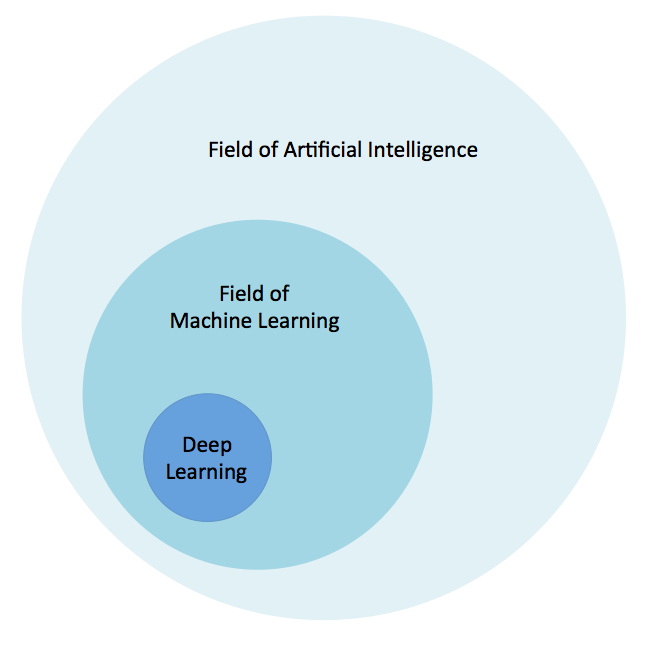
\includegraphics[width=8cm]{figs/ai-ml-dl-relationship.png}
	\caption{Relación entre Inteligencia Artificial, Machine Learning y Deep Learning}
	\label{fig:ai-ml-dl}
\end{figure}

El \textit{Deep Learning} se diferencia del \textit{Machine Learning} convencional, en que están formados por modelos con distintas ramas de procesamiento que son capaces de extraer las representaciones de los datos con varios niveles de abstracción \cite{lecun2015deep}. Mucha de la teoría relacionada se puede encontrar en los años 50 y 60, sin embargo, las aplicaciones y la capacidad de cómputo eran limitadas en la época, hasta ahora donde la capacidad de computación ha crecido a gran escala y en conjunto con las nuevas técnicas propuestas, una mayor cantidad de datos y la aplicación de transformaciones no lineales hacen que esta vertiente viva su época dorada.

Una de las implementaciones más representativas del \textit{Deep Learning} se trata de las redes neuronales, las cuales se encuentran basadas en el funcionamiento del cerebro humano, utilizando el concepto de neuronas que pueden realizar cálculos, la conexión entre las mismas, la función de realizar una tarea específica, etc. Añadir, que se encuentra basado y que el cerebro humano es un sistema mucho más complejo que las redes neuronales y tiene muchos más comportamientos \cite{haykin1994neural}.


Dentro del \textit{Machine Learning}, los algoritmos pueden dividirse según como se realice el entrenamiento del modelo, afectando también a la evaluación y las aplicaciones del mismo. Estas categorias son: \textit{Aprendizaje Supervisado (Supervised Learning), Aprendizaje No Supervidado (Unsupervised Learning) y Aprendizaje Semi-Supervisado (Semi-Supervised Learning)}

\subsection{Aprendizaje Supervisado}

El aprendizaje supervisado se caracteriza por utilizar un conjunto de variables de entrada y encontrar la función que más se aproxime a los valores de salida \cite{Liu2012}. Actualmente es una de las metodologías más utilizadas en \textit{Machine Learning} y es una de las más avanzadas en el campo, sin embargo, la necesidad de los valores de salida (variable dependiente o \textit{target}) requiere que el conjunto de datos se encuentre etiquetado, es decir, para las observaciones de las variables de entrada debe existir la variable de salida para poder general el modelo. En muchos casos este etiquetado se debe de realizar manualmente, por lo que es un proceso que requiere mucho tiempo.

Por otro lado, cabe mencionar que el uso de métodos de aprendizaje supervisado tienen una mayor efectividad que el semi y no supervisado, sin embargo, la necesidad de tener las etiquetas y el coste que ello supone para grandes cantidades de datos, como es en el caso de la detección de anomalías, provocan que se busquen otras soluciones con aprendizajes semi y no supervisado. Además, suele suceder que en la detección de anomalías, éstas sean la menor parte de todos los datos, en otras palabras, la mayor parte de los datos son normales y solo una pequeña porción se trata de anomalías como tal, provocando que el conjunto de datos esté poco compensado.

Uno de los modelos más sencillos de aprendizaje supervisado es la regresión lineal (simple), ésta permite ajustar a una serie de puntos conocidos , \textit{x}, y su respuesta \textit{y} \cite{james2013introduction}, generando una función que permite predecir los valores de \textit{y} con valores no conocidos de \textit{x}:

\begin{equation}
y = ax + b 
\end{equation}

En este caso se predicen los nuevos valores utilizando la función ajustada, existen distintos métodos para encontrar la recta que ajusta los puntos, siendo uno de los más utilizados el ajuste por mínimos cuadrados:

\begin{equation}
a = \frac{\sum(x_i – \bar{x}) (y_i – \bar{y})} {\sum(x_i – \bar{x})^2}
\end{equation}

\begin{equation}
b = y – a \bar{x}
\end{equation}

\begin{figure}[H]
	\centering
	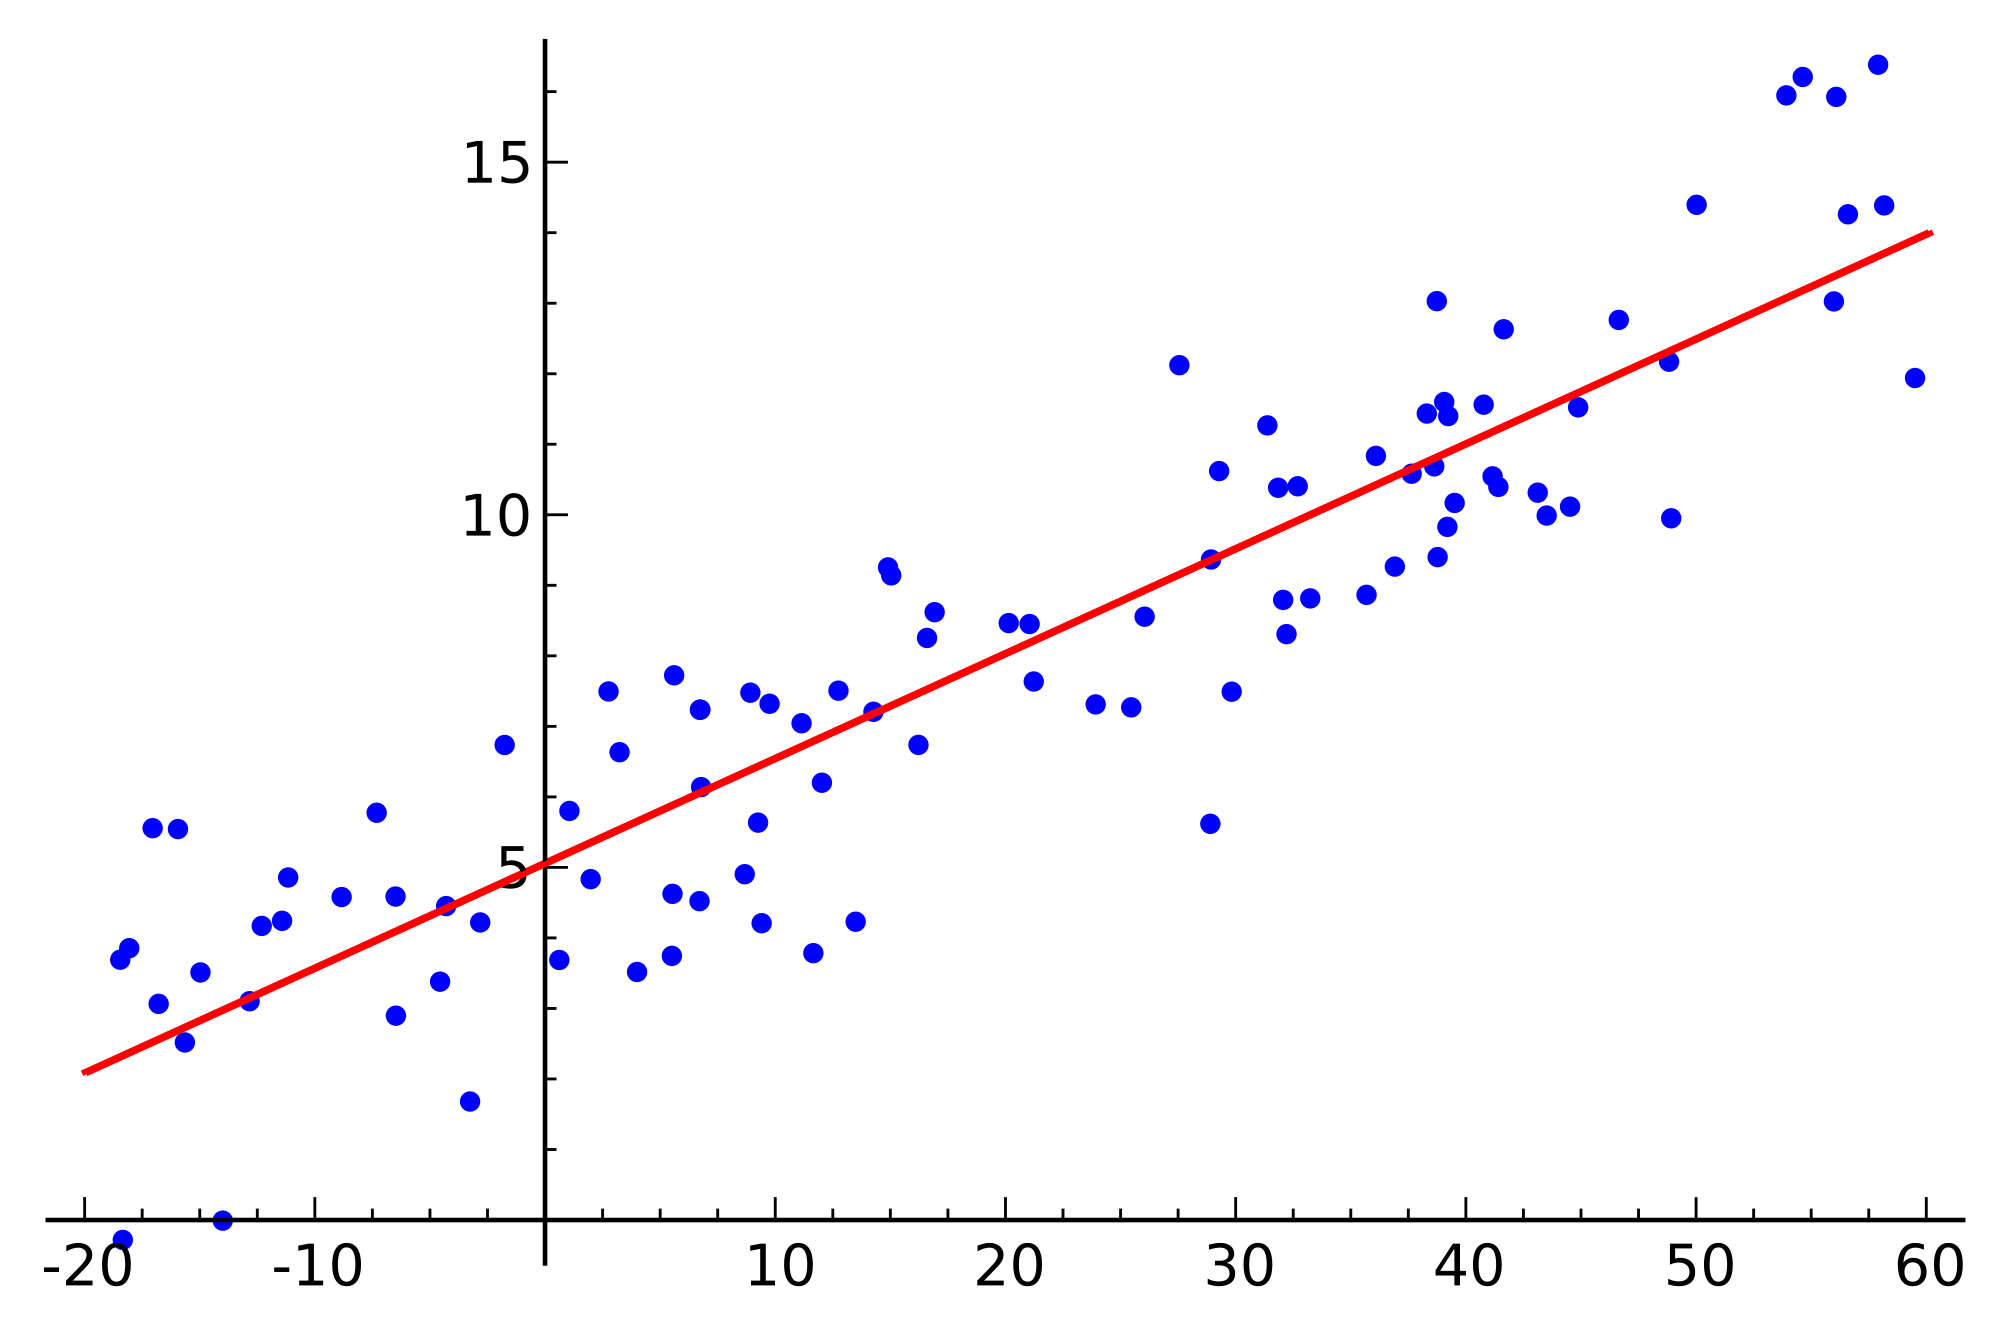
\includegraphics[width=8cm]{figs/Linear_regression.png}
	\caption{Regresión Lineal}
	\label{fig:reglin}
\end{figure}

Como se puede observar en la imagen \ref{fig:reglin}, se ha generado una recta capaz de ajustarse a los puntos y predecir el valor para nuevos puntos. Para generar la función de la recta se ha necesita utilizar la variable dependiente \textit{y} en el entrenamiento para poder generar la función que aproximará los nuevos puntos. 

Durante los siguientes apartados se van a mostrar los distintos modelos utilizados en aprendizaje supervisado para la detección de anomalías, como las redes neuronales artificiales (\textit{Artificial Neural Networks, ANN}, \textit{Gradient Boosting Machines} y \textit{Support Vector Machines}

\subsubsection{Feedforwark Neural Network}

Tal y como se ha comentado anteriormente, las redes neuronales intentan imitar el concepto de la conexión de neuronas del cerebro humano, éstas están formadas por una capa de entrada de datos (\textit{Input}), una capa de salida (\textit{Input}) y un conjunto de capas intermedias, también llamadas capas ocultas (\textit{Hidden}) \cite{haykin1994neural}. En las capas intermedias se encuentran las neuronas conectadas entre sí y pueden estar formadas desde una sola capa, hasta \textit{n} capas, sin embargo, cuanto mayor sea el número de capas, mayor coste de computación asociado. En la siguiente imagen \ref{fig:ANN} podemos ver como sería una arquitectura de una red neuronal:

\begin{figure}[H]
	\centering
	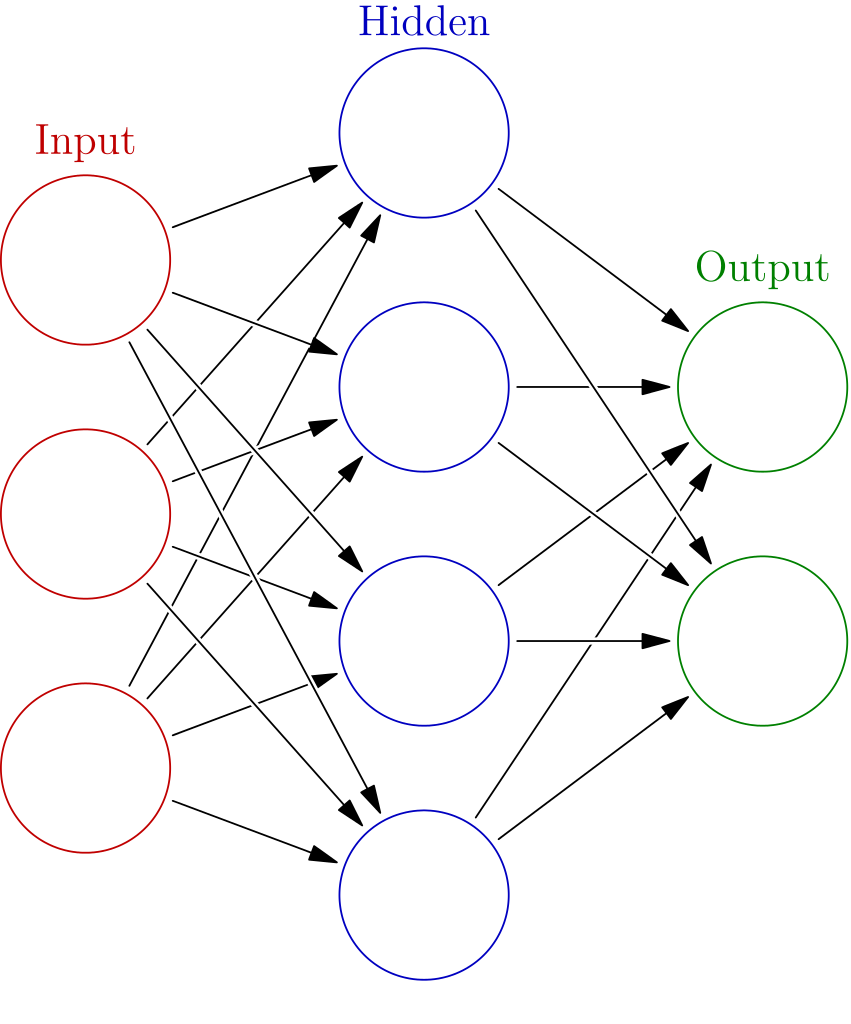
\includegraphics[width=8cm]{figs/Colored_neural_network.png}
	\caption{Red Neuronal Artificial}
	\label{fig:ANN}
\end{figure}

Dentro de las redes neuronales existe un caso base conocido como perceptron, un clasificador binario formado por la capa de entrada, una capa oculta de una sola neurona y una salida \cite{rosenblatt1958perceptron}. El perceptrón ayudará a incluir el concepto de los pesos (\textit{weights}) y el \textit{bias}. 

\begin{figure}[H]
	\centering
	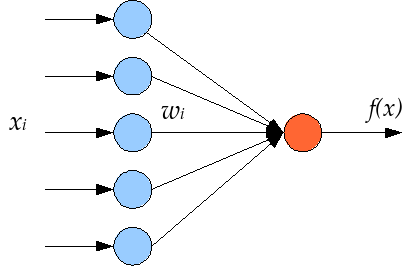
\includegraphics[width=8cm]{figs/Single_layer_perceptron.png}
	\caption{Arquitectura de un Perceptron}
	\label{fig:perceptron}
\end{figure}

Los valores de entrada \(X\) son multiplicados por una serie de pesos \(W\), en una primera instancia se inician aleatoriamente, y se realiza la suma de esta multiplicación, tras la cual se pasará a una función de activación. La función de activación define el valor de salida de la neurona y que se utilizará como valor de entrada para la siguiente neurona o como es en este caso como el valor de salida final. Un ejemplo de una función de activación es la función escalón, donde los valores menores de cero son iguales a cero y los mayores de cero son igual a uno. El \textit{bias} se trata de un pequeño valor que modifica el output sin interactura con las neuronas. De este modo la clasificación de 0 o 1 en un perceptron sería así:

\begin{equation}
    f(x) = g(\sum XW + b)
\end{equation}

Donde \(g(x)\) es la función de activación, X el vector de datos de entrada, W el vector de pesos y b el vector de bias.

\begin{figure}[H]
	\centering
	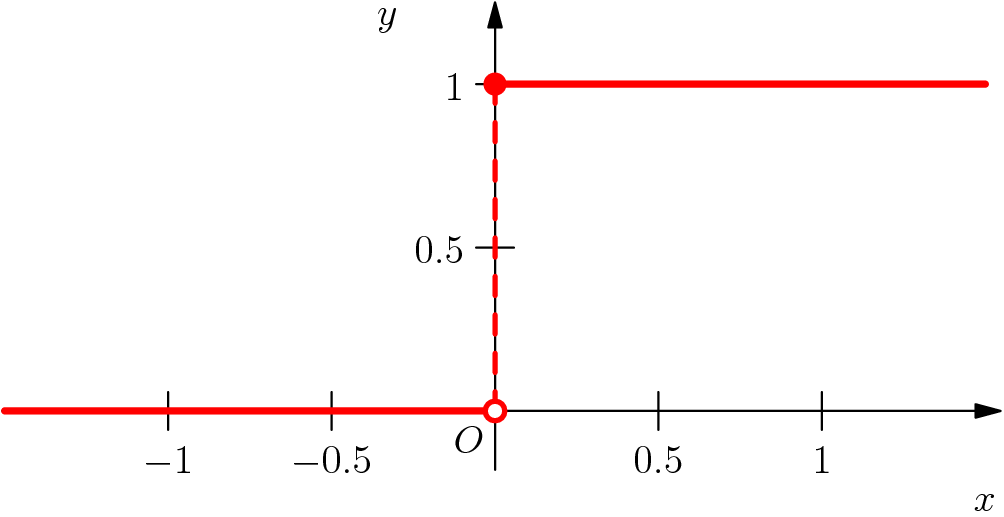
\includegraphics[width=8cm]{figs/stepfunction.png}
	\caption{Función de activación: Función Escalón}
	\label{fig:stepfunction}
\end{figure}

Aumentando la complejidad de la arquitectura, es decir, el número de neuronas, el numero de capas y distintas funciones de activación, se consiguen modelos más complejos pero mantienen el enfoque que se realiza en el perceptron.

Para optimizar la salida, se utilizan varias técnicas de optimización que permiten actualizar los pesos \(W\) y disminuir el error \(E = f(x) - y\), una de las más utilizadas es el \textit{backpropagation}, basado en el descenso del gradiente cuyo objetivo es obtener el gradiente de la función (vector de mayor pendiente) pero utilizar el valor opuesto del mismo multiplicado por un coeficiente de aprendizaje (\textit{learning rate}), una anlogía muy utilizada es imaginar como encontrar el punto más bajo del valle, para ello lo mejor es fijarse en que lugar del punto en el que nos encontremos tiene más pendiente negativa y seguir ese camino. El backpropagation utiliza esté método, pero en lugar de calcular el gradiente sobre la función total (gran coste) se realiza el cálculo de los gradientes locales, empezando desde el punto final de la función.

\begin{figure}[H]
    \centering
    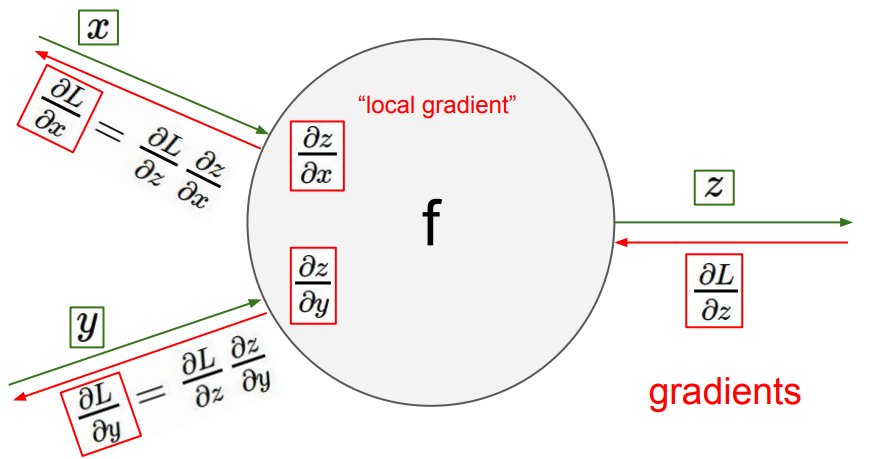
\includegraphics[width=8cm]{figs/backprop.png}
    \caption{Backpropagation}
    \label{fig:backprop}
\end{figure}

La fórmula de la actualización de los pesos en una ANN sería similar a la siguiente:
\begin{equation}
    W_i+1 = W_i - \gamma \frac{1}{n} \sum \nabla L(x,w)
\end{equation}

Donde \(\gamma\) es el \textit{learning rate} y \(L(x)\) es la función de pérdida.

La última capa, la capa de \textit{outputs}, define el número de neuronas de salida, que puede ser igual al número de clases etiquetadas o una sola neurona en el caso de que existan solo dos clases, clasificación binaria. El valor de las salidas irá definido por la función de activación de la última capa de la capa oculta.

\subsubsection{Gradient Boosting Machines}

Las \textit{Gradient Boosting Machines} son uno de los métodos más utilizados actualmente, dada la gran precisión que aportan a la resolución de los problemas. Estos modelos se basan en realizar el ensamblado de modelos débiles, normalmente árboles de decisión, para generar un predictor "fuerte" de una manera iterativa. 

\subsubsection{Support Vector Machines}

\subsection{Aprendizaje No Supervisado}
\subsubsection{Long Short Term Memory Networks}
\subsubsection{Autoencoders}
\subsubsection{Generative Adversarial Networks}
\subsubsection{Recurrent Neural Networks}

\subsection{Aprendizaje Semi-Supervisado}
\subsubsection{Autoencoders}
\subsubsection{Convolutional Neural Networks}
\subsubsection{Generative Adversarial Networks}

% bibliografia
\addcontentsline{toc}{chapter}{Bibliografía}
\bibliographystyle{unsrt}
\bibliography{referencias}

\end{document}